\documentclass[12pt]{report}
\input{etc/cmd}
\usepackage{float}
\usepackage{tikz}
\usetikzlibrary{positioning}
\usepackage{amsmath}
\usepackage{amsfonts}
\usepackage{amssymb}
\usepackage{polyglossia}
\setmainlanguage{farsi}
\setotherlanguage{english}
\settextfont{XB Yas.ttf}
\setlatintextfont{times.ttf}

\begin{document}
\fontsize{12pt}{14pt}\selectfont

\input{etc/head}
\renewcommand{\thesection}{\arabic{section}}

\section{بخش ۱}


\section{پیاده‌سازی دستی الگوریتم Isomap}

در این بخش، الگوریتم \lr{Isomap} را بدون استفاده از توابع آماده‌ی کتابخانه‌ها مانند \lr{scikit-learn} پیاده‌سازی کرده‌ایم. هدف اصلی، درک بهتر مراحل الگوریتم و مقایسه نتایج آن با نسخه‌ی کتابخانه‌ای است.

\subsection{ساخت گراف $k$-نزدیک‌ترین همسایه‌ها}

ابتدا برای هر نقطه، $k$ تا از نزدیک‌ترین نقاط دیگر را با استفاده از فاصلهٔ اقلیدسی پیدا می‌کنیم. برای این کار:

\begin{itemize}
    \item یک ماتریس فاصله \lr{(Distance Matrix)} بین تمامی نمونه‌ها محاسبه می‌کنیم.
    \item سپس برای هر سطر، $k$ مقدار کوچک‌تر (غیر صفر) را نگه می‌داریم.
    \item مقادیر دیگر را برابر با بی‌نهایت (\(\infty\)) قرار می‌دهیم تا مسیر مستقیم بین آن نقاط در گراف قطع شود.
\end{itemize}

این کار منجر به ساخت گرافی می‌شود که تنها یال‌های مربوط به $k$ همسایه‌ی نزدیک هر نقطه را شامل می‌شود.

\subsection{محاسبه‌ی فاصله‌های ژئودزیک با الگوریتم Floyd-Warshall}

برای تخمین فاصله‌ی ژئودزیک بین هر دو نقطه، از الگوریتم \lr{Floyd-Warshall} استفاده کردیم که برای گراف‌های وزن‌دار جهت‌دار مناسب است. این الگوریتم برای تمامی جفت گره‌ها، کوتاه‌ترین مسیر را محاسبه می‌کند.

\begin{itemize}
    \item ورودی: ماتریس وزن‌دار گراف (با $\infty$ برای یال‌های غیرفعال)
    \item خروجی: ماتریس فاصله‌ی ژئودزیک بین همه‌ی جفت نقاط
\end{itemize}

\subsection{کاهش بُعد با استفاده از MDS}

پس از محاسبهٔ ماتریس فاصله‌ی ژئودزیک، از \lr{Multidimensional Scaling (MDS)} برای نگاشت داده‌ها به فضای دوبعدی استفاده کردیم. مراحل انجام MDS به شرح زیر است:

\begin{enumerate}
    \item محاسبه‌ی ماتریس فاصله‌ی مربعی \( D^{2} \) با استفاده از فواصل ژئودزیک.
    \item مرکزسازی داده‌ها با استفاده از ماتریس \( H = I - \frac{1}{n}ee^T \) و محاسبه‌ی:
    \[
    B = -\frac{1}{2} H D^{2} H
    \]
    \item انجام تجزیه‌ی مقادیر ویژه روی ماتریس $B$ و استخراج بردارهای ویژه متناظر با دو مقدار ویژه بزرگ‌تر برای نگاشت دوبعدی.
\end{enumerate}


\subsection{چرخش و بازتاب نگاشت Isomap}


برای هماهنگ‌سازی جهت‌گیری نگاشت \lr{Isomap} با نقشه‌های جغرافیایی متداول، دو گام زیر انجام شده است:



به زبان ریاضی:
\[
\begin{aligned}
(x_{\mathrm{rot}}, y_{\mathrm{rot}})
&= (-\,y,\,x),\\
(x_{\mathrm{final}}, y_{\mathrm{final}})
&= (-\,x_{\mathrm{rot}},\,y_{\mathrm{rot}})
= (y,\,x).
\end{aligned}
\]

این تبدیل باعث می‌شود که جهت‌های شرقی–غربی و شمالی–جنوبی در نگاشت نهایی با انتظار ما از نقشه‌های جغرافیایی هم‌راستا شوند (شرق به راست و شمال به بالا).

\subsection{تفسیر نگاشت پس از چرخش}

شکل زیر نگاشت دوبعدی شهرهای ایران را پس از چرخش و بازتاب نشان می‌دهد:

\begin{figure}[H]
  \centering
  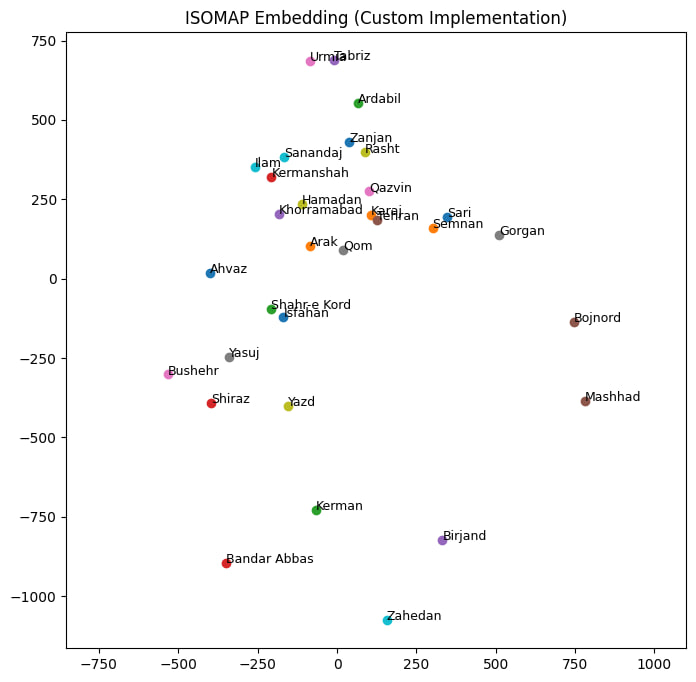
\includegraphics[width=0.8\textwidth]{custom_isomap.jpg}
  \caption{نگاشت \lr{Isomap} پس از چرخش و بازتاب}
  \label{fig:isomap-rotated}
\end{figure}

\begin{itemize}
  \item \textbf{شمال غرب:} شهرهای \lr{Tabriz} و \lr{Urmia} در بالای نگاشت و اندکی به چپ قرار دارند.
  \item \textbf{شمال شرق:} شهرهای \lr{Ardabil} و \lr{Zanjan} در بالا و راست متمرکز شده‌اند.
  \item \textbf{مرکز:} \lr{Tehran}, \lr{Qom} و \lr{Arak} نزدیک مرکز قرار گرفته‌اند که نشان‌دهندهٔ کانون جغرافیایی ایران است.
  \item \textbf{جنوب غرب:} شهرهای \lr{Bushehr}, \lr{Shiraz} و \lr{Yasuj} در نیمهٔ پایین و سمت چپ نگاشت واقع شده‌اند.
  \item \textbf{جنوب شرق:} \lr{Zahedan} و \lr{Birjand} در پایین و راست نگاشت دیده می‌شوند.
\end{itemize}

این چینش نشان‌دهندهٔ حفظ ساختار ژئودزیک (فاصله‌های زمینی بر اساس کوتاه‌ترین مسیر در گراف همسایگی) توسط الگوریتم \lr{Isomap} است و نزدیکی‌های جغرافیایی شهرها را به خوبی در فضای کم‌بعد منعکس می‌کند.

\subsection{نتیجه ایزومپ کتابخانه \lr{sklearn}}


نتیجه‌ی حاصل از تحلیل پراکرستس بین نگاشت دوبُعدی پیاده‌سازی‌شده‌ی دستی و نگاشت حاصل از کتابخانه‌ی \lr{sklearn} برابر با صفر است \lr{(Procrustes disparity = 0.000000)}. این مقدار نشان‌دهنده‌ی هم‌پوشانی کامل و دقیق بین این دو نگاشت، پس از اعمال تبدیل‌های ایزومتریک (مانند دوران، انتقال و بازتاب) است. به عبارت دیگر، ساختار کلی داده‌ها در فضای کم‌بعدی در هر دو پیاده‌سازی به‌صورت یکسان حفظ شده است و تفاوتی از نظر هندسه‌ی نسبی نقاط وجود ندارد. این نتیجه دقت بالای پیاده‌سازی دستی الگوریتم \lr{ISOMAP} را تأیید می‌کند.



\begin{figure}[H]
  \centering
  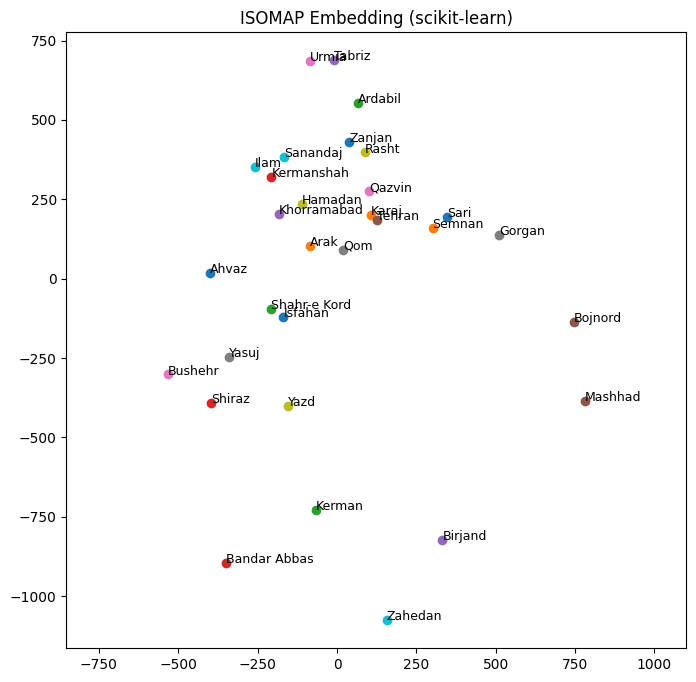
\includegraphics[width=0.8\textwidth]{sklearn_isomap.png}
  \caption{خروجی \lr{sklearn} پس از اعمال نگاشت چرخش}

\end{figure}


\section{بخش ۲: سوالات تشریحی}

\subsection{سوال ۱}
  از تعریف کوواریانس داریم:
  \[
  \Sigma=\frac{1}{m-1}X^{T}X.
  \]
  با جایگذاری تجزیهٔ مقدار تکین $X=USV^{T}$:
  \[
  X^{T}X = (USV^{T})^{T}(USV^{T})
        = VS^{T}U^{T}USV^{T}.
  \]
  از آن‌جا که $U$ متعامد است، $U^{T}U=I$، بنابراین:
  \[
  X^{T}X = VS^{T}SV^{T}.
  \]
  پس:
  \[
  \Sigma=\frac{1}{m-1}VS^{T}SV^{T}.
  \]
  اکنون توجه کنید که $S$ یک ماتریس قطری-مستطیلی است. اگر رتبهٔ $X$ برابر $r$ باشد، می‌توان نوشت:
  \[
  S=
  \begin{bmatrix}
  \operatorname{diag}(s_{1},\dots,s_{r}) & 0\\
  0 & 0
  \end{bmatrix},
  \qquad s_{1}\ge \cdots \ge s_{r}>0,
  \]
  که در آن $s_i$ها مقادیر تکین $X$ هستند. در این حالت،
  \[
  S^{T}S=
  \begin{bmatrix}
  \operatorname{diag}(s_{1}^{2},\dots,s_{r}^{2}) & 0\\
  0 & 0
  \end{bmatrix}
  \in\mathbb{R}^{n\times n}.
  \]
  پس می‌توان $\Sigma$ را به‌صورت یک تجزیهٔ ویژه نوشت:
  \[
  \Sigma
  =V\left(\frac{1}{m-1}S^{T}S\right)V^{T}.
  \]
  از آن‌جا که $V$ متعامد است و ماتریس $\frac{1}{m-1}S^{T}S$ قطری و با درایه‌های غیرمنفی است، نتیجه می‌شود:

  \begin{itemize}
  \item \textbf{بردارهای ویژهٔ $\Sigma$} برابر ستون‌های $V$ هستند (یعنی $v_i$ها).
  \item \textbf{مقادیر ویژهٔ $\Sigma$} برابر مربع مقادیر تکین تقسیم بر $(m-1)$ هستند:
  \[
  \lambda_i(\Sigma)=\frac{s_i^{2}}{m-1},\qquad i=1,\dots,r,
  \]
  و برای $i>r$ (در صورت $r<n$) داریم $\lambda_i(\Sigma)=0$.
  \end{itemize}

  برای مشاهدهٔ مستقیم، اگر $V=[v_1,\dots,v_n]$ باشد، آنگاه:
  \[
  \Sigma v_i
  =\frac{1}{m-1}VS^{T}SV^{T}v_i
  =\frac{1}{m-1}VS^{T}Se_i
  =\frac{s_i^{2}}{m-1}v_i,
  \]
  که نشان می‌دهد $v_i$ بردار ویژه و $\frac{s_i^2}{m-1}$ مقدار ویژه متناظر است.






  \subsection{سوال ۲}

  \subsection*{صورت‌بندی هندسیِ تصویر و خطا}
فرض کنید $u\in\mathbb{R}^n$ یک بردار \textbf{یکه} باشد ($\|u\|_2=1$). تصویر عمودیِ $x_i$ روی زیرفضای یک‌بُعدیِ $\operatorname{span}(u)$ برابر است با:
\[
F(x_i)=\hat x_i = (u^{T}x_i)\,u.
\]
بردار خطای بازسازی (مولفهٔ عمود بر زیرفضا) نیز:
\[
e_i = x_i - \hat x_i = x_i - (u^{T}x_i)u.
\]

\subsection*{۱) هم‌ارزیِ بیشینه‌سازی طول تصویر و کمینه‌سازی خطا}
چون $\hat x_i$ تصویر عمودی روی $\operatorname{span}(u)$ است، داریم $\hat x_i \perp e_i$ و لذا از قضیهٔ فیثاغورس:
\[
\|x_i\|_2^2 = \|\hat x_i\|_2^2 + \|e_i\|_2^2.
\]
از طرفی چون $\|u\|_2=1$:
\[
\|\hat x_i\|_2^2=\|(u^{T}x_i)u\|_2^2=(u^{T}x_i)^2\,\|u\|_2^2=(u^{T}x_i)^2.
\]
پس برای هر $i$:
\[
\|e_i\|_2^2 = \|x_i\|_2^2 - (u^{T}x_i)^2.
\]
اکنون مجموع خطای بازسازی (معیار رایجِ کمینه‌سازی در \lr{PCA}) را در نظر بگیرید:
\[
J(u)=\sum_{i=1}^{m}\|e_i\|_2^2
=\sum_{i=1}^{m}\|x_i\|_2^2-\sum_{i=1}^{m}(u^{T}x_i)^2.
\]
چون داده‌ها ثابت‌اند، عبارت $\sum_{i=1}^{m}\|x_i\|_2^2$ مستقل از $u$ است؛ بنابراین:
\[
\arg\min_{\|u\|_2=1} J(u)
=
\arg\max_{\|u\|_2=1}\sum_{i=1}^{m}(u^{T}x_i)^2.
\]
اما $\sum_{i=1}^{m}(u^{T}x_i)^2$ دقیقاً مجموعِ مربعِ «طول تصویر اسکالر» روی $u$ است. همچنین چون داده‌ها مرکزسازی شده‌اند، میانگین $u^{T}x_i$ صفر است و واریانس تصویرهای اسکالر $y_i=u^{T}x_i$ برابر است با:
\[
\operatorname{Var}(y)=\frac{1}{m-1}\sum_{i=1}^{m}(u^{T}x_i)^2.
\]
پس بیشینه‌کردن $\sum_{i}(u^{T}x_i)^2$ معادل بیشینه‌کردن واریانسِ داده‌های تصویرشده است. نتیجه:
\[
\boxed{\;
\text{بیشینه‌سازی واریانس تصویرها}
\;\Longleftrightarrow\;
\text{کمینه‌سازی خطای بازسازی (کمترین مربعات).}
\;}
\]

\subsection*{بیان ماتریسی (رابطه با کوواریانس)}
اگر $X\in\mathbb{R}^{m\times n}$ ماتریس داده‌های مرکزسازی‌شده باشد (سطرها نمونه‌ها)، آنگاه:
\[
\sum_{i=1}^{m}(u^{T}x_i)^2 = \|Xu\|_2^2 = u^{T}X^{T}Xu.
\]
با تعریف کوواریانس نمونه‌ای
\[
\Sigma=\frac{1}{m-1}X^{T}X,
\]
داریم:
\[
\operatorname{Var}(Xu)=\frac{1}{m-1}\|Xu\|_2^2 = u^{T}\Sigma u.
\]
پس مسئلهٔ بیشینه‌سازی واریانس به شکل کلاسیکِ ریلی (\lr{Rayleigh quotient}) درمی‌آید:
\[
\max_{\|u\|_2=1} u^{T}\Sigma u,
\]
که جواب آن بردار ویژهٔ متناظر با بزرگ‌ترین مقدار ویژهٔ $\Sigma$ است.

\subsection*{۲) نتیجه دربارهٔ اطلاعات از دست‌رفته در کاهش بعد}
از رابطهٔ فیثاغورس برای هر نمونه:
\[
\|x_i\|_2^2 = \|\hat x_i\|_2^2 + \|e_i\|_2^2,
\]
و با جمع روی همهٔ نمونه‌ها:
\[
\sum_{i=1}^{m}\|x_i\|_2^2
=
\sum_{i=1}^{m}\|\hat x_i\|_2^2
+
\sum_{i=1}^{m}\|e_i\|_2^2.
\]
یعنی «انرژی کل داده» بین «انرژیِ نگه‌داشته‌شده در زیرفضای انتخابی» و «انرژیِ باقیمانده/از‌دست‌رفته» تقسیم می‌شود. بنابراین در \lr{PCA}، زیرفضای بهینه طوری انتخاب می‌شود که:
\begin{itemize}
\item بیشترین سهم از واریانس (انرژی) را نگه دارد؛
\item و معادل آن، کمترین انرژی را در مولفه‌های حذف‌شده باقی بگذارد (کمترین خطای بازسازی).
\end{itemize}
پس \textbf{اطلاعات از دست‌رفته} دقیقاً برابر با انرژی/واریانسِ مؤلفه‌های عمود بر زیرفضای انتخاب‌شده است؛ در حالت کلی $k$ مؤلفه، این مقدار برابر مجموع مقادیر ویژهٔ حذف‌شده است:
\[
\text{واریانسِ از دست‌رفته}=\sum_{j=k+1}^{n}\lambda_j(\Sigma),
\qquad
\text{واریانسِ حفظ‌شده}=\sum_{j=1}^{k}\lambda_j(\Sigma),
\]
که در آن $\lambda_1\ge\cdots\ge\lambda_n\ge 0$ مقادیر ویژهٔ کوواریانس هستند.

\subsection{سوال ۳}

\subsection*{(الف) هم‌راستایی تقریبی \lr{PC1} با کدام ویژگی؟}
در \lr{PCA} (وقتی از ماتریس کوواریانس استفاده می‌شود)، جهتِ $\text{PC1}$ جهتی است که \textbf{واریانس تصویر داده‌ها روی آن بیشینه} شود؛ یعنی بیشترین سهم از انرژی/پراکندگی داده را پوشش دهد.

وقتی هیچ استانداردسازی انجام نشده باشد، \textbf{مقیاس عددی ویژگی‌ها} تعیین می‌کند کدام ویژگی بیشترین واریانس را وارد ماتریس کوواریانس می‌کند. در دادهٔ حاضر:
\begin{itemize}
\item \textbf{شناسهٔ کاربر} یک عدد ترتیبی با مقیاس حدود $10^6$ است (واریانس بزرگ، اما از نظر معنایی \underline{بی‌ربط}).
\item \textbf{درآمد سالیانه} حتی از شناسه هم در مقیاس بسیار بزرگ‌تری است (تا مرتبهٔ $10^{10}$).
\item سن، زمان حضور و نرخ تبدیل در مقیاس‌های بسیار کوچک‌تر هستند (ده‌ها، صدها، یا صدم‌ها).
\end{itemize}

بنابراین، بدون محاسبهٔ دقیق، انتظار می‌رود $\text{PC1}$ تقریباً با \textbf{یکی از ویژگی‌های دارای بزرگ‌ترین واریانس عددی} هم‌راستا شود؛ در این مسئله معمولاً \textbf{درآمد سالیانه} (و در بسیاری از پیاده‌سازی‌های خام حتی \textbf{شناسهٔ کاربر} اگر پراکندگی آن زیاد باشد) می‌تواند غالب شود. نکتهٔ کلیدی این است که \textbf{PC1 تحت سلطهٔ مقیاس} قرار می‌گیرد، نه اهمیت معنایی.

\paragraph{آیا این مؤلفه برای دسته‌بندی مشتریان ارزشمند است؟}
اگر $\text{PC1}$ عمدتاً توسط \textbf{شناسهٔ کاربر} شکل گرفته باشد، از دید تحلیل رفتار مشتری \textbf{تقریباً بی‌ارزش} است؛ چون شناسه یک برچسب ترتیبی است و ساختار هندسیِ معنی‌دار از رفتار یا ترجیح ایجاد نمی‌کند (فقط عددی بزرگ است). اگر هم $\text{PC1}$ عمدتاً درآمد را پوشش دهد، ممکن است برای \textbf{تفکیک اقتصادی} تا حدی مفید باشد، اما هنوز مشکل اصلی پابرجاست: سایر ویژگی‌های رفتاری (نرخ تبدیل، زمان حضور، سن) به علت مقیاس کوچک‌تر، در مؤلفه‌های ابتدایی کم‌رنگ می‌شوند و فضای \lr{PCA} ممکن است برای هدف توصیه‌گر، «نمایندهٔ رفتار» نباشد \cite{Jolliffe}.

\subsection*{(ب) سرنوشت نرخ تبدیل در \lr{PCA} خام}
نرخ تبدیل در بازهٔ $0.01$ تا $0.05$ تغییر می‌کند؛ یعنی تغییرات آن در مقیاس «صدم» است. در مقابل، درآمد یا شناسه در مقیاس‌های میلیون تا ده‌میلیارد نوسان دارند. از آن‌جا که \lr{PCA} بدون نظارت است و فقط \textbf{واریانس} را بیشینه می‌کند، ویژگی‌هایی با واریانس کوچک معمولاً:
\begin{itemize}
\item یا در \textbf{مؤلفه‌های با رتبهٔ بالاتر} (مثلاً $\text{PC4},\text{PC5},\dots$) ظاهر می‌شوند،
\item یا اگر با ویژگی‌های بزرگ‌مقیاس هم‌بستگی قوی نداشته باشند، سهم کمی در $\text{PC1--PC3}$ خواهند داشت.
\end{itemize}

پس حتی اگر نرخ تبدیل از نظر کسب‌وکار «مهم‌ترین» ویژگی برای وفاداری باشد، در \lr{PCA} خام (بدون نرمال‌سازی/استانداردسازی) احتمال زیادی وجود دارد که \textbf{اثر آن در سه مؤلفهٔ اول دیده نشود}؛ زیرا معیار انتخاب مؤلفه‌ها «اطلاعات مفید برای وفاداری» نیست، بلکه «بیشترین واریانس عددی» است

\paragraph{نتیجهٔ عملی}
برای آن‌که نرخ تبدیل واقعاً در مؤلفه‌های اولیه نقش بگیرد، باید از پیش‌پردازش‌های متداول مانند \textbf{استانداردسازی} (مثلاً \lr{z-score}) یا استفاده از \textbf{ماتریس هم‌بستگی} به‌جای کوواریانس استفاده شود تا هر ویژگی سهمی هم‌تراز از مقیاس داشته باشد.

\subsection*{(ج) چرا تغییر واحد زمان (ثانیه به میکروثانیه) ساختار \lr{PC}ها را عوض می‌کند؟}
فرض کنید داده‌ها مرکزسازی شده‌اند و ستون پنجم (زمان حضور) را در ماتریس $X$ با ضریب
\[
\alpha = 10^{6}
\]
مقیاس کنیم (چون $1\text{ s}=10^{6}\text{ }\mu\text{s}$). یعنی ستون پنجم جدید:
\[
x_{(5)}' = \alpha\, x_{(5)}.
\]
اگر $D$ یک ماتریس قطری باشد که همهٔ درایه‌های قطری آن ۱ هستند به‌جز درایهٔ پنجم که $\alpha$ است، آنگاه:
\[
X' = X D.
\]
اکنون کوواریانس نمونه‌ای (طبق صورت سؤال) برابر است با:
\[
S = \frac{1}{n-1}X^{T}X,
\qquad
S' = \frac{1}{n-1}{X'}^{T}X' = \frac{1}{n-1}D^{T}X^{T}XD = D^{T} S D.
\]
چون $D$ قطری و $D^{T}=D$ است:
\[
S' = D S D.
\]
بنابراین:
\begin{itemize}
\item درایهٔ قطریِ مربوط به ویژگی پنجم (واریانس زمان) \textbf{با ضریب $\alpha^2$} بزرگ می‌شود:
\[
\operatorname{Var}(x_{(5)}') = \alpha^{2}\operatorname{Var}(x_{(5)}).
\]
\item کوواریانس‌های بین زمان و سایر ویژگی‌ها \textbf{با ضریب $\alpha$} مقیاس می‌شوند:
\[
\operatorname{Cov}(x_{(5)}',x_{(j)}')=\alpha\,\operatorname{Cov}(x_{(5)},x_{(j)}),\quad j\neq 5.
\]
\end{itemize}

از آن‌جا که مقادیر ویژه و بردارهای ویژهٔ $S$ با این تغییر مقیاس عوض می‌شوند، \textbf{جهت‌های \lr{PC}} نیز تغییر می‌کنند. اگر $\alpha$ بسیار بزرگ باشد (مثل $10^{6}$)، ستون پنجم می‌تواند به‌قدری غالب شود که:
\begin{itemize}
\item یکی از بزرگ‌ترین مقدارهای ویژه تقریباً به واریانسِ ستون پنجم نسبت داده شود،
\item و بردار ویژهٔ متناظر، تقریباً در راستای محور زمان قرار گیرد،
\end{itemize}
در نتیجه «یک مؤلفهٔ اصلی که تقریباً فقط زمان را می‌بیند» ظاهر می‌شود. این دقیقاً همان حساسیت \lr{PCA} به \textbf{واحد و مقیاس} در نسخهٔ مبتنی بر کوواریانس است .


تغییر مقیاسِ یک ویژگی معمولاً فقط «یک مؤلفه» را تغییر نمی‌دهد؛ \textbf{کل طیف مقادیر/بردارهای ویژه} می‌تواند جابه‌جا شود. اما وقتی یک ستون به‌شدت غالب شود، معمولاً یک جهتِ غالب (اغلب $\text{PC1}$ یا یکی از \text{PC}های ابتدایی) عملاً به همان ویژگی قفل می‌شود و سایر مؤلفه‌ها مجبور می‌شوند در زیرفضای عمود بر آن تنظیم شوند.


\end{document}
